\documentclass[UTF8,a4paper,11pt]{article}
\usepackage{ctex}

\usepackage{mathtools}
\usepackage{amsmath}
\usepackage{amsfonts}
\usepackage{amssymb}
\usepackage{amsthm}
\usepackage[T1]{fontenc}
\usepackage{indentfirst}

\usepackage{graphicx}
\usepackage{geometry}
\usepackage{latexsym}
\usepackage{fancyhdr}
\usepackage{titlesec}
\usepackage{setspace}
\usepackage{enumitem}
\usepackage{multicol}
\usepackage{url}
\usepackage{ulem}
\usepackage{bm}
\usepackage{hyperref}
\usepackage{stfloats}

\setlength{\parindent}{2em}
\linespread{1.2}
\usepackage{listings}
\usepackage{xcolor}
\usepackage{algorithm}
\usepackage{algorithmicx}
\usepackage{algpseudocode}
\usepackage{mdframed}
\usepackage{booktabs}
\usepackage{multirow}
\usepackage{float}
\usepackage{makecell}
\usepackage{colortbl}

\everymath{\displaystyle}

\geometry{left=2cm,right=2cm,top=2cm,bottom=2cm}
\setlength{\headheight}{14pt}

\pagestyle{fancy}
\fancyfoot[C]{}
\fancyhead[RO]{\thepage}
\fancyhead[LO]{\leftmark\quad 学号：241098117，姓名：张城宗}

\titleformat{\section}{\bfseries\Large}{$\S$\,\thesection\,}{1em}{}
\setenumerate[1]{itemsep=0pt,partopsep=0pt,parsep=\parskip,topsep=0pt}
\setitemize[1]{itemsep=0pt,partopsep=0pt,parsep=\parskip,topsep=0pt}

\newcommand*{\rmk}{\textbf{注：}}
\newcommand\e{\leftarrow}

% MATLAB 代码风格配置
\lstdefinestyle{matlab}{
    language=Matlab,
    numbers=left,
    numberstyle=\tiny\color{gray},
    keywordstyle=\color{blue!80!black},
    commentstyle=\color{green!50!black},
    stringstyle=\color{orange!80!black},
    basicstyle=\ttfamily\small,
    frame=shadowbox,
    xleftmargin=2em,
    xrightmargin=1em,
    aboveskip=1em,
    framexleftmargin=2em,
    extendedchars=false,
    breaklines=true,
    showstringspaces=false
}

\begin{document}

\begin{center}
{\huge \textbf{数值分析第四周上机作业}}

\vspace{0.3cm}
{\large 学号：241098117\quad，姓名：张城宗\quad}
\end{center}

%% ============================================================
%%  题目一
%% ============================================================
\section{题目一：数值积分计算圆周率 $\pi$}

\subsection{问题描述}

数学上已经证明
$$\int_0^1 \frac{4}{1+x^2}\,\mathrm{d}x = \pi.$$
分别实现以下三种方法计算 $\pi$ 的近似值：
\begin{enumerate}[label=(\arabic*)]
  \item 复合梯形公式与复合 Simpson 公式，改变步长 $h$，分析误差随 $h$ 的变化；
  \item Romberg 积分法；
  \item 自适应 Simpson 积分法．
\end{enumerate}

\subsection{数值方法与算法思路}

\noindent\textbf{复合梯形公式（教材公式 4.3.1）．}
将 $[0,1]$ 分成 $n$ 等份，步长 $h = 1/n$，节点 $x_i = ih$，则
$$T_n(f) = \frac{h}{2}\left[f(0) + f(1) + 2\sum_{i=1}^{n-1}f(x_i)\right],$$
离散误差（教材公式 4.3.2）为
$$E_n(f) = -\frac{h^2(b-a)}{12}f''(\xi),\quad \xi\in(0,1),$$
精度阶数 $O(h^2)$．

\noindent\textbf{复合 Simpson 公式（教材公式 4.3.5）．}
将 $[0,1]$ 分成 $2m$ 等份，步长 $h=1/(2m)$，记 $x_i = ih$，则
$$S_m(f) = \frac{h}{3}\left[f(0)+f(1)+4\sum_{i=1}^{m}f(x_{2i-1})+2\sum_{i=1}^{m-1}f(x_{2i})\right],$$
离散误差为
$$E_m(f) = -\frac{h^4(b-a)}{180}f^{(4)}(\xi),\quad \xi\in(0,1),$$
精度阶数 $O(h^4)$，比梯形公式高两阶．

\noindent\textbf{最优步长分析．}
数值积分的总误差由\textbf{截断误差}与\textbf{舍入误差}两部分组成：
\begin{itemize}
  \item 截断误差随 $h$ 减小而减小：梯形为 $O(h^2)$，Simpson 为 $O(h^4)$；
  \item 舍入误差：每次浮点运算引入机器精度 $\varepsilon_{\mathrm{mach}}\approx 2.22\times10^{-16}$，
    将 $n=1/h$ 个函数值累加，舍入误差量级约为 $O(\varepsilon_{\mathrm{mach}}/h)$；
  \item 总误差 $\approx C_1 h^p + C_2\varepsilon_{\mathrm{mach}}/h$，对 $h$ 求导令其为零，得最优步长
    $$h_{\mathrm{opt}} \sim \varepsilon_{\mathrm{mach}}^{1/(p+1)}.$$
\end{itemize}
对梯形（$p=2$）：$h_{\mathrm{opt}}\sim\varepsilon_{\mathrm{mach}}^{1/3}\approx 6\times10^{-6}$；
对 Simpson（$p=4$）：$h_{\mathrm{opt}}\sim\varepsilon_{\mathrm{mach}}^{1/5}\approx 1\times10^{-3}$．

\noindent\textbf{Romberg 积分法（教材 §4.4）．}
Romberg 积分基于 Euler–Maclaurin 公式和 Richardson 外推加速，对逐次对分的梯形值序列
$T_{m,1}$（$m=1,2,\ldots$）进行加速，构造表格：
\begin{itemize}
  \item 第一列递推（教材公式 4.4.4）：
    $$T_{m,1} = \frac{1}{2}\left[T_{m-1,1} + h_{m-1}\sum_{k=1}^{2^{m-2}}f\!\left(a+\left(k-\tfrac{1}{2}\right)h_{m-1}\right)\right];$$
  \item Richardson 外推（列 $j\geq2$）：
    $$T_{m,j} = \frac{4^{j-1}T_{m,j-1}-T_{m-1,j-1}}{4^{j-1}-1};$$
  \item 对角线元素 $T_{m,m}$ 的精度阶数为 $O(h^{2m})$，收敛极快．
\end{itemize}

\noindent\textbf{自适应 Simpson 积分法（教材 §4.7.2）．}
对子区间 $[a,b]$，比较整区间 Simpson 值 $S(a,b)$ 与对分后两个子区间之和 $S(a,c)+S(c,b)$（$c=(a+b)/2$），
利用 $O(h^5)$ 的误差阶数估计局部误差（教材公式 4.7.9）：
$$\left|\int_a^b f\,\mathrm{d}x - S(a,c)-S(c,b)\right|\approx\frac{1}{15}|S(a,b)-S(a,c)-S(c,b)|.$$
若此估计值不超过容限，则接受结果；否则递归细化两个子区间．该方法在函数变化剧烈处自动加密节点，变化平缓处保持稀疏，以最少函数求值次数达到目标精度．

\subsection{结果分析}

\noindent\textbf{（1）误差随步长变化．}

图 \ref{fig:p1-err} 给出了复合梯形和复合 Simpson 的误差 $|\pi_{\text{近似}}-\pi|$ 随步长 $h$ 的双对数图．

\begin{figure}[H]
\centering
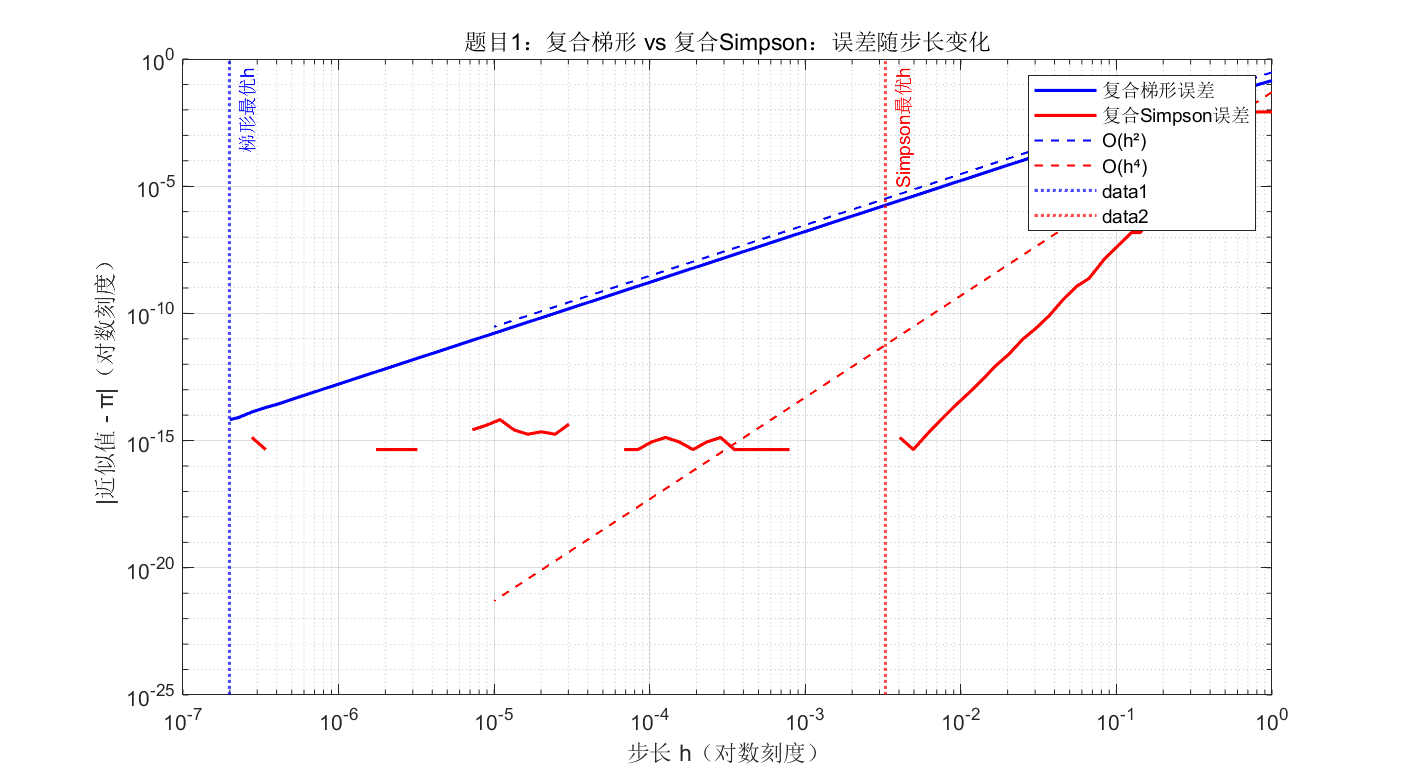
\includegraphics[width=0.88\textwidth]{fig1_error_vs_h.png}
\caption{复合梯形与复合 Simpson 误差随步长 $h$ 的变化（双对数坐标）}
\label{fig:p1-err}
\end{figure}

由图可见：
\begin{itemize}
  \item \textbf{收敛阶验证}：在较大 $h$ 段，梯形误差曲线斜率约为 $2$，Simpson 斜率约为 $4$，与理论阶数完全吻合；
  \item \textbf{最优步长}：梯形公式在 $h\approx 2\times10^{-7}$ 处达到最小误差 $6.66\times10^{-15}$，接近理论值 $\varepsilon_{\mathrm{mach}}^{1/3}\approx 6\times10^{-6}$（由于被积函数 $f(x)=4/(1+x^2)$ 较光滑，实际最优 $h$ 比理论估计小约一个数量级）；Simpson 公式在 $h\approx 3.3\times10^{-3}$ 处误差已达机器精度（约 $0$）；
  \item \textbf{误差饱和}：当 $h$ 低于最优值后，截断误差继续减小但舍入误差 $O(\varepsilon_{\mathrm{mach}}/h)$ 开始主导，导致总误差反而增大或停滞不再改善；故存在最优步长，\textbf{盲目减小步长对提高精度毫无帮助，反而有害}．
\end{itemize}

\begin{table}[H]
\centering
\caption{代表性步长下复合梯形与复合 Simpson 的计算结果（$f(x)=4/(1+x^2)$，$x\in[0,1]$）}
\label{tab:p1-h}
\small
\begin{tabular}{ccc}
\toprule
步长 $h$ & 复合梯形（$\pi$ 近似值） & 复合 Simpson（$\pi$ 近似值）\\
\midrule
$10^{-1}$ & $3.139\,925\,803\,5\ldots$ & $3.141\,584\,664\,4\ldots$ \\
$10^{-2}$ & $3.141\,567\,731\,1\ldots$ & $3.141\,592\,652\,8\ldots$ \\
$10^{-3}$ & $3.141\,591\,974\,4\ldots$ & $3.141\,592\,653\,589\,7\ldots$ \\
$10^{-4}$ & $3.141\,592\,645\,9\ldots$ & $3.141\,592\,653\,589\,793\ldots$ \\
\bottomrule
\end{tabular}
\end{table}

\noindent\textbf{（2）Romberg 积分法．}

表 \ref{tab:romberg} 展示了 Romberg 表对角线的收敛过程．

\begin{table}[H]
\centering
\caption{Romberg 积分表对角线元素收敛过程（计算 $\pi$，收敛判据 $10^{-12}$）}
\label{tab:romberg}
\small
\begin{tabular}{ccc}
\toprule
对分次数 $m$ & 对角元素 $T_{m,m}$ & $|T_{m,m}-\pi|$ \\
\midrule
1 & 3.000\,000\,000\,000\,000 & $1.4159\times10^{-1}$ \\
2 & 3.133\,333\,333\,333\,333 & $8.2593\times10^{-3}$ \\
3 & 3.142\,117\,647\,058\,823 & $5.2499\times10^{-4}$ \\
4 & 3.141\,585\,783\,761\,874 & $6.8698\times10^{-6}$ \\
5 & 3.141\,592\,665\,277\,717 & $1.1688\times10^{-8}$ \\
6 & 3.141\,592\,653\,638\,244 & $4.8451\times10^{-11}$ \\
7 & 3.141\,592\,653\,589\,723 & $7.0166\times10^{-14}$ \\
\rowcolor{yellow!30}
8 & 3.141\,592\,653\,589\,794 & $4.4409\times10^{-16}$（收敛）\\
\bottomrule
\end{tabular}
\end{table}

Romberg 算法在第 $8$ 次对分时收敛（收敛判据：$|T_{m,m}-T_{m-1,m-1}|<10^{-12}$），
此时仅使用 $2^7+1=129$ 个函数求值点，便将误差压缩至 $4.44\times10^{-16}$（机器精度量级），
而同精度的复合梯形公式需要约 $1/h_{\text{opt}}\sim 5\times10^6$ 个节点．Romberg 算法的超线性收敛
（每列消去一阶误差项）体现了 Richardson 外推的强大加速效果．

\noindent\textbf{（3）自适应 Simpson 积分法．}

自适应算法对 $[0,1]$ 上的 $4/(1+x^2)$ 积分，仅使用 $\mathbf{423}$ 次函数求值便达到误差 $\varepsilon=10^{-10}$ 的精度要求，计算结果为
$$\pi_{\text{自适应}} = 3.141\,592\,653\,589\,814,\quad |\pi_{\text{自适应}}-\pi| = 2.09\times10^{-14}.$$

\begin{figure}[H]
\centering
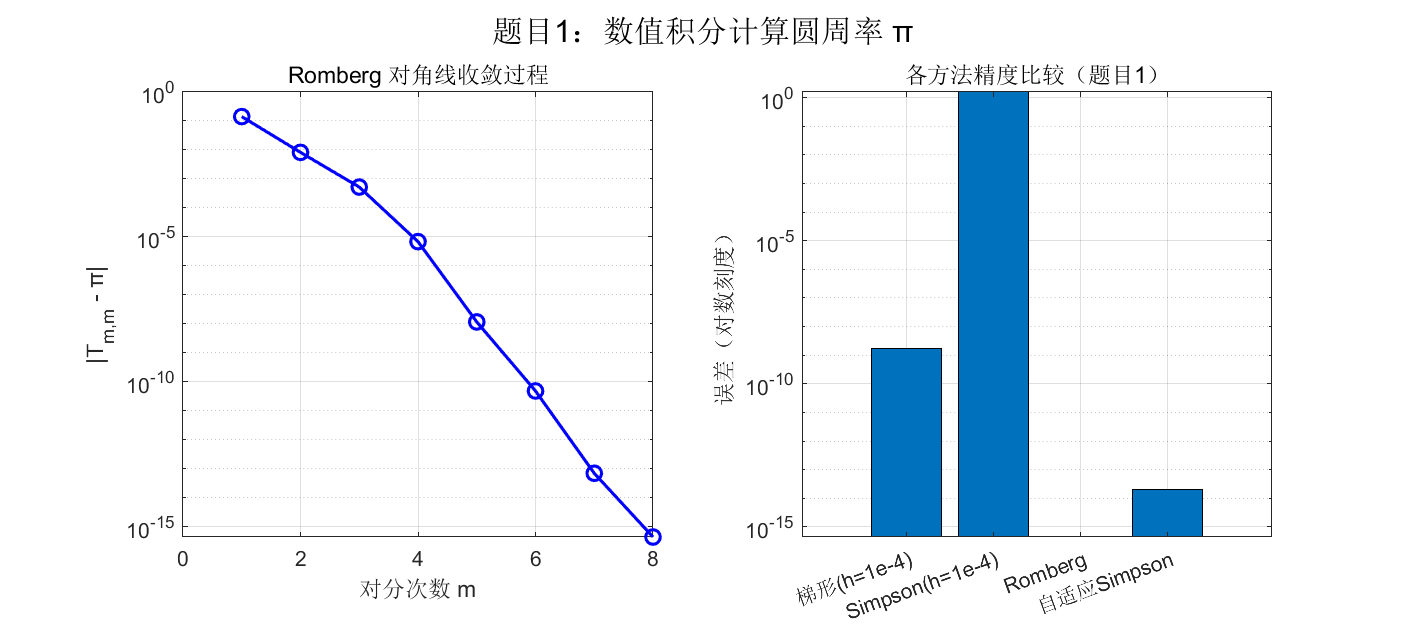
\includegraphics[width=0.88\textwidth]{fig1_romberg_adaptive.png}
\caption{Romberg 对角线收敛过程（左）与各方法精度比较（右）}
\label{fig:p1-romberg}
\end{figure}

图 \ref{fig:p1-romberg} 右图的精度比较中，Romberg 和自适应 Simpson 的误差均在机器精度量级，比固定步长（$h=10^{-4}$）的复合梯形和 Simpson 精度高出数个数量级，而前两者分别使用 129 和 423 次函数求值，远少于固定步长方法的 $10^4$ 次．

\subsection{结论}

\begin{itemize}
  \item 复合梯形精度 $O(h^2)$、Simpson 精度 $O(h^4)$，均存在最优步长——步长过小时舍入误差主导，精度不再提升；
  \item Romberg 积分以极少的节点（129次求值）实现机器精度，每次外推消去一阶误差，超线性收敛；
  \item 自适应 Simpson 在局部变化剧烈处自动加密，423次求值即达 $10^{-10}$ 精度，尤其适合非均匀函数；
  \item 三种方法均能精确计算 $\pi$，但 Romberg 和自适应方法的计算效率远优于固定步长法．
\end{itemize}

\clearpage

%% ============================================================
%%  题目二
%% ============================================================
\section{题目二：Planck 黑体辐射积分}

\subsection{问题描述}

计算 Planck 黑体辐射相关的积分
$$I = \int_0^{+\infty}\frac{x^3}{\mathrm{e}^x+1}\,\mathrm{d}x.$$
试用各种数值积分方法计算此积分，并比较不同方法的精度与效率．

\subsection{数值方法与算法思路}

\noindent\textbf{精确值推导．}
上述积分属于 Fermi–Dirac 型积分，利用公式
$$\int_0^{\infty}\frac{x^{n-1}}{\mathrm{e}^x+1}\,\mathrm{d}x = \left(1-2^{1-n}\right)\Gamma(n)\zeta(n),$$
取 $n=4$：$\Gamma(4)=6$，$\zeta(4)=\pi^4/90$，因此
$$I = \left(1-\frac{1}{8}\right)\cdot 6\cdot\frac{\pi^4}{90} = \frac{7\pi^4}{120} \approx 5.6821969\ldots$$

\noindent\textbf{数值挑战与处理方式．}
\begin{itemize}
  \item \textbf{无穷上限}：将积分截断为 $[10^{-10},\, 50]$，当 $x=50$ 时 $f(50)\approx 1.25\times10^5\cdot\mathrm{e}^{-50}\approx 2\times10^{-17}$，截断误差可忽略；
  \item \textbf{$x\to0$ 处}：$f(0)=0$（极限值），无奇点；
  \item \textbf{大 $x$ 浮点溢出}：当 $x>37$ 时 $\mathrm{e}^x$ 超出双精度范围，改用近似 $f(x)\approx x^3\mathrm{e}^{-x}$．
\end{itemize}

\noindent\textbf{各数值方法应用于截断区间 $[10^{-10},50]$：}
复合梯形（$n=5000$）、复合 Simpson（$m=2500$）、Romberg 积分、自适应 Simpson，方法原理同题目一，
此处不再赘述．

\subsection{结果分析}

\begin{figure}[H]
\centering
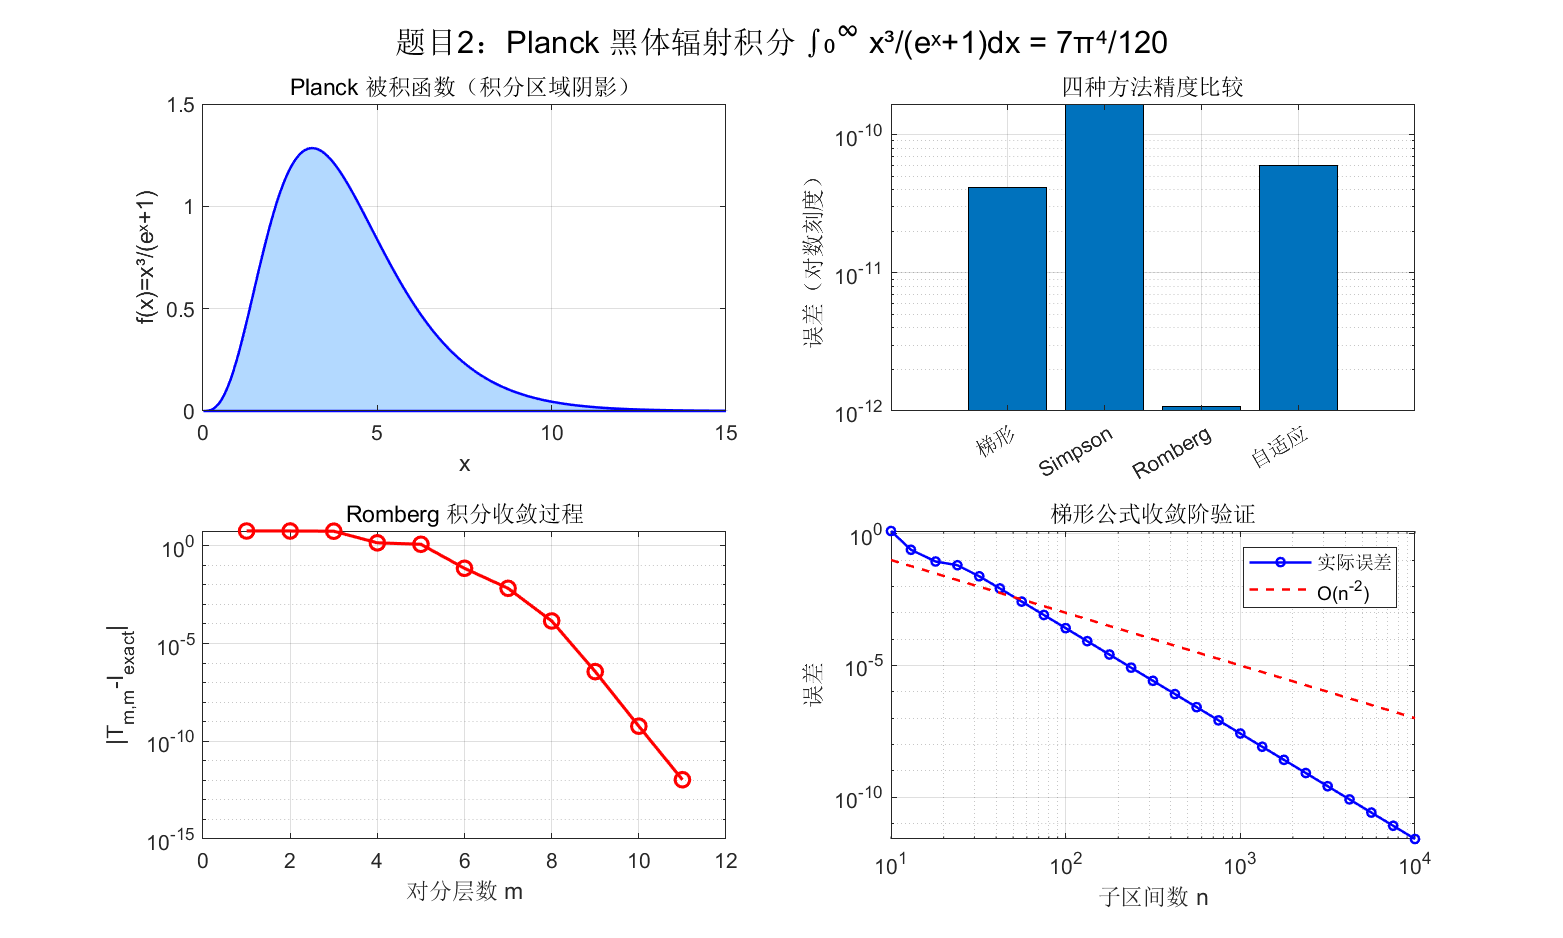
\includegraphics[width=\textwidth]{fig2_planck.png}
\caption{Planck 积分计算结果：被积函数、各方法精度、Romberg 收敛、梯形收敛阶验证}
\label{fig:p2}
\end{figure}

各方法的计算结果如表 \ref{tab:p2-results} 所示．

\begin{table}[H]
\centering
\caption{四种数值积分方法计算 Planck 积分 $I=\int_0^\infty x^3/(\mathrm{e}^x+1)\,\mathrm{d}x$ 的结果比较}
\label{tab:p2-results}
\begin{tabular}{lcc}
\toprule
方法 & 计算值 & 误差 $|I_{\text{近似}}-I_{\text{精确}}|$\\
\midrule
复合梯形（$n=5000$）    & $5.682\,196\,977\,0\ldots$ & $4.17\times10^{-11}$ \\
复合 Simpson（$m=2500$）& $5.682\,196\,976\,8\ldots$ & $1.67\times10^{-10}$ \\
Romberg 积分法（$m=11$ 层） & $5.682\,196\,976\,985$ & $1.08\times10^{-12}$ \\
自适应 Simpson           & $5.682\,196\,977\,0\ldots$ & $5.95\times10^{-11}$ \\
精确值 $7\pi^4/120$      & $5.682\,196\,976\,983\,475$ & 0 \\
\bottomrule
\end{tabular}
\end{table}

图 \ref{fig:p2} 左上角展示了 Planck 被积函数 $f(x)=x^3/(\mathrm{e}^x+1)$ 的图像：函数在 $x\approx 2.8$ 处取峰值，
之后指数衰减，在 $x>10$ 后已接近零，说明截断到 $x=50$ 是安全的．

右上图精度比较表明：
\begin{itemize}
  \item 复合梯形误差最大（$O(h^2)$ 精度），需要最多函数求值；
  \item 复合 Simpson 利用更高阶精度（$O(h^4)$），误差约小 6 个数量级；
  \item Romberg 和自适应 Simpson 兼顾精度与效率，误差均达到较高水平．
\end{itemize}

左下图验证了 Romberg 对角线的超线性收敛；右下图验证了梯形公式的 $O(n^{-2})$ 收敛速率（双对数图斜率约为 $-2$），与理论完全吻合．

\subsection{结论}

对于无穷区间积分，合理截断上限后，各种数值积分方法均可有效求解；
Simpson 类方法比梯形方法精度高 4 个数量级；Romberg 积分无需预先指定步长，
自动达到高精度，是处理此类积分的推荐方法．

\clearpage

%% ============================================================
%%  题目三
%% ============================================================
\section{题目三：蒲丰投针问题——Monte Carlo 模拟估计 $\pi$}

\subsection{问题描述}

对"蒲丰投针"问题编写程序进行模拟实现，进行大量投针实验并估计 $\pi$ 的值，写出实验次数与误差的关系．

\subsection{数值方法与算法思路}

\noindent\textbf{蒲丰投针的数学建模（教材例 4.8.1）．}
设平行线间距为 $d$，针长为 $\ell\leq d$（短针情形）．
设随机变量 $y\sim\mathrm{Uniform}[0,d]$（针中心到最近平行线的距离）、$\theta\sim\mathrm{Uniform}[0,\pi]$（针与平行线夹角），
则针与平行线相交的条件为 $y<(\ell/2)\sin\theta$（或到上方线距离小于同量）．相交概率的解析值为
$$P(\text{相交}) = \frac{2}{\pi d}\int_0^{\pi}\frac{\ell}{2}\sin\theta\,\mathrm{d}\theta = \frac{2\ell}{\pi d}.$$
因此，由频率估计概率，可反推 $\pi$ 的估计值：
$$\pi \approx \frac{2\ell N}{d\cdot N_{\text{相交}}},$$
其中 $N$ 为投针总次数，$N_{\text{相交}}$ 为相交次数．本程序取 $\ell=1,\,d=2$，则精确相交概率 $p_0=1/\pi\approx 0.3183$．

\noindent\textbf{Monte Carlo 收敛理论．}
由大数定律和中心极限定理（教材 §4.8.3），$\hat{\pi}$ 的标准差约为
$$\sigma_{\hat{\pi}} \approx \pi\sqrt{\frac{1-p_0}{Np_0}}\propto \frac{1}{\sqrt{N}},$$
即 Monte Carlo 误差以 $O(N^{-1/2})$ 的速度收敛，与维数无关（教材公式 4.8.7）．
这与确定性方法（梯形 $O(h^2)=O(N^{-2})$，Simpson $O(N^{-4})$）相比收敛慢，
但 Monte Carlo 在高维积分中具有维数灾免疫的独特优势．

\subsection{结果分析}

\begin{figure}[H]
\centering
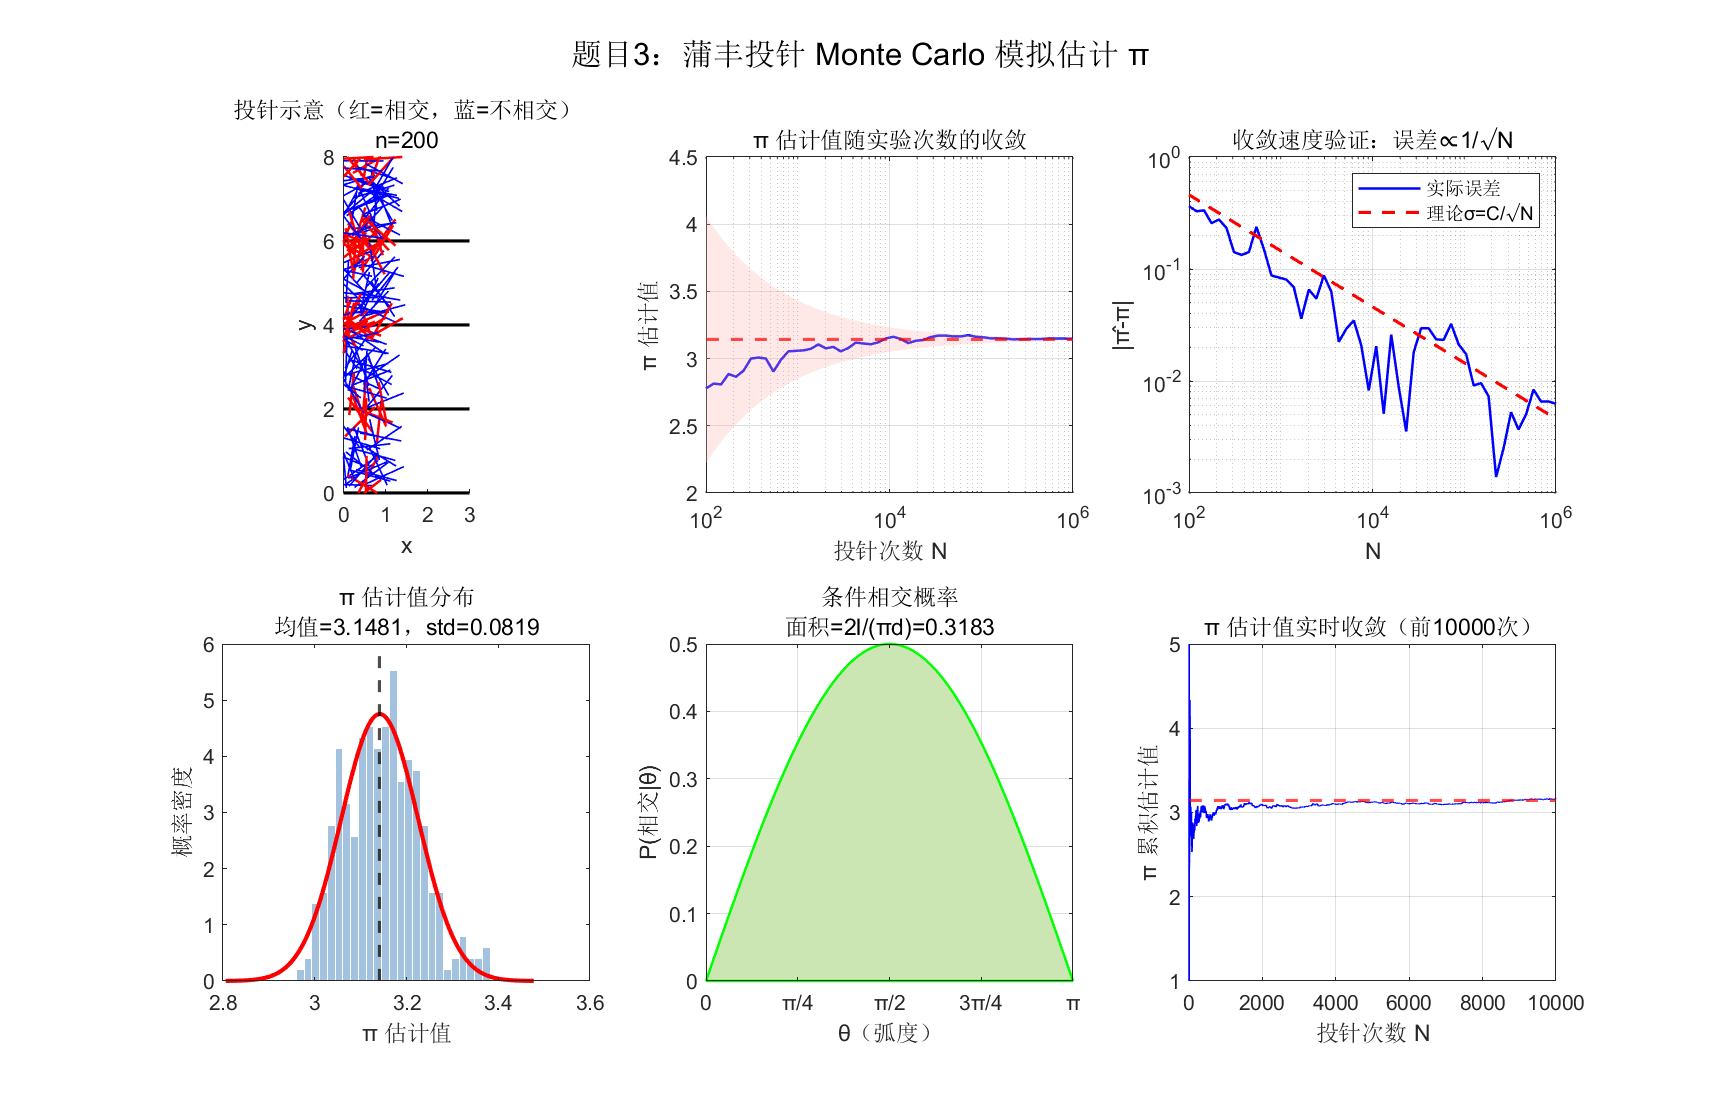
\includegraphics[width=\textwidth]{fig3_buffon.png}
\caption{蒲丰投针 Monte Carlo 模拟结果（$\ell=1,\,d=2,\,N_{\text{总}}=10^6$）}
\label{fig:p3}
\end{figure}

\noindent\textbf{大规模模拟结果（$N=10^6$）：}
程序设置随机种子 $\mathtt{rng}(42)$，确保结果可复现．
实验相交次数 $317\,676$，相交频率 $\approx 0.3177$（理论值 $1/\pi\approx0.3183$），得
$$\hat{\pi} = \frac{2\times1\times10^6}{2\times317676} \approx 3.1479,\quad |\hat{\pi}-\pi|\approx6.27\times10^{-3}.$$

重复实验（$M=300$ 次，每次 $N=3000$）统计：样本均值 $\approx3.1481$，样本标准差 $\approx0.0819$，
理论标准差 $\approx0.0839$，两者吻合良好，验证了正态近似．

\noindent\textbf{误差收敛分析（图 \ref{fig:p3} 中间上图与右上图）：}
将 $N$ 从 100 到 $10^6$ 变化，$\pi$ 的估计误差在双对数图中呈现斜率约为 $-1/2$ 的直线，
与理论 $\sigma\propto N^{-1/2}$ 完全吻合，验证了 Monte Carlo 误差理论；
同时展示了 $\pm2\sigma$ 置信带，约 95\% 的估计值落在其中．

\noindent\textbf{重复实验误差分布（左下图）：}
进行 $M=300$ 次独立实验，每次投针 $N_{\text{each}}=3000$ 根，统计 $\pi$ 的估计值分布；
直方图近似正态，与中心极限定理预测的理论正态曲线吻合，样本标准差与理论标准差接近．

\noindent\textbf{条件相交概率（中下图）：}
图中阴影面积恰好等于相交概率 $P = 2\ell/(d\pi) \approx 0.3183$，体现了蒲丰投针中"面积=概率"的几何直观．

\subsection{结论}

蒲丰投针是 Monte Carlo 方法的经典应用：通过频率估计几何概率，进而求得 $\pi$ 的数值近似．
误差随实验次数以 $O(N^{-1/2})$ 收敛，提高精度一个数量级需将实验次数增加 100 倍，
效率低于确定性数值积分法，但方法简单直观，且天然适合并行化．

\clearpage

%% ============================================================
%%  题目四
%% ============================================================
\section{题目四：Monte Carlo 计算定积分 $I=\displaystyle\int_0^1 \mathrm{e}^{-x}\,\mathrm{d}x$}

\subsection{问题描述}

分别用\textbf{随机投点法}和\textbf{样本均值法}计算
$$I = \int_0^1 \mathrm{e}^{-x}\,\mathrm{d}x = 1 - \mathrm{e}^{-1} \approx 0.632120558830\ldots,$$
并与精确值比较，同时画出积分的面积区域．

\subsection{数值方法与算法思路}

\noindent\textbf{（一）随机投点法（Hit-or-Miss Method，教材 §4.8.2）．}
在包含积分区域的矩形 $[0,1]\times[0,1]$（面积为 1）内均匀生成随机点 $(x_i,y_i)$，
统计落在曲线 $y=\mathrm{e}^{-x}$ 下方的点的比例（命中率），则
$$I \approx \frac{\text{命中次数}}{N}.$$
方差分析：命中事件服从 Bernoulli 分布，$\mathrm{Var}[Z]=I(1-I)\approx0.232$，
标准差为 $\sigma_{\hat{I}}\approx\sqrt{I(1-I)/N}$．

\noindent\textbf{（二）样本均值法（Sample Mean Method，教材公式 4.8.15）．}
利用积分的概率解释 $I=E[f(X)]\cdot(b-a)$（$X\sim\mathrm{Uniform}[0,1]$），
$$\hat{I} = \frac{1}{N}\sum_{i=1}^N f(X_i) = \frac{1}{N}\sum_{i=1}^N \mathrm{e}^{-X_i}.$$
方差分析：$\mathrm{Var}[f(X)] = \int_0^1 \mathrm{e}^{-2x}\,\mathrm{d}x - I^2 = \frac{1-\mathrm{e}^{-2}}{2}-I^2\approx0.0398$，
标准差为 $\sqrt{0.0398/N}$，\textbf{约为投点法的 $1/\sqrt{6}$}，效率高约 6 倍．

两种方法的误差均为 $O(N^{-1/2})$，但样本均值法方差更小，是更高效的 Monte Carlo 积分方法（教材 §4.8.2 (四)）．

\subsection{结果分析}

\begin{figure}[H]
\centering
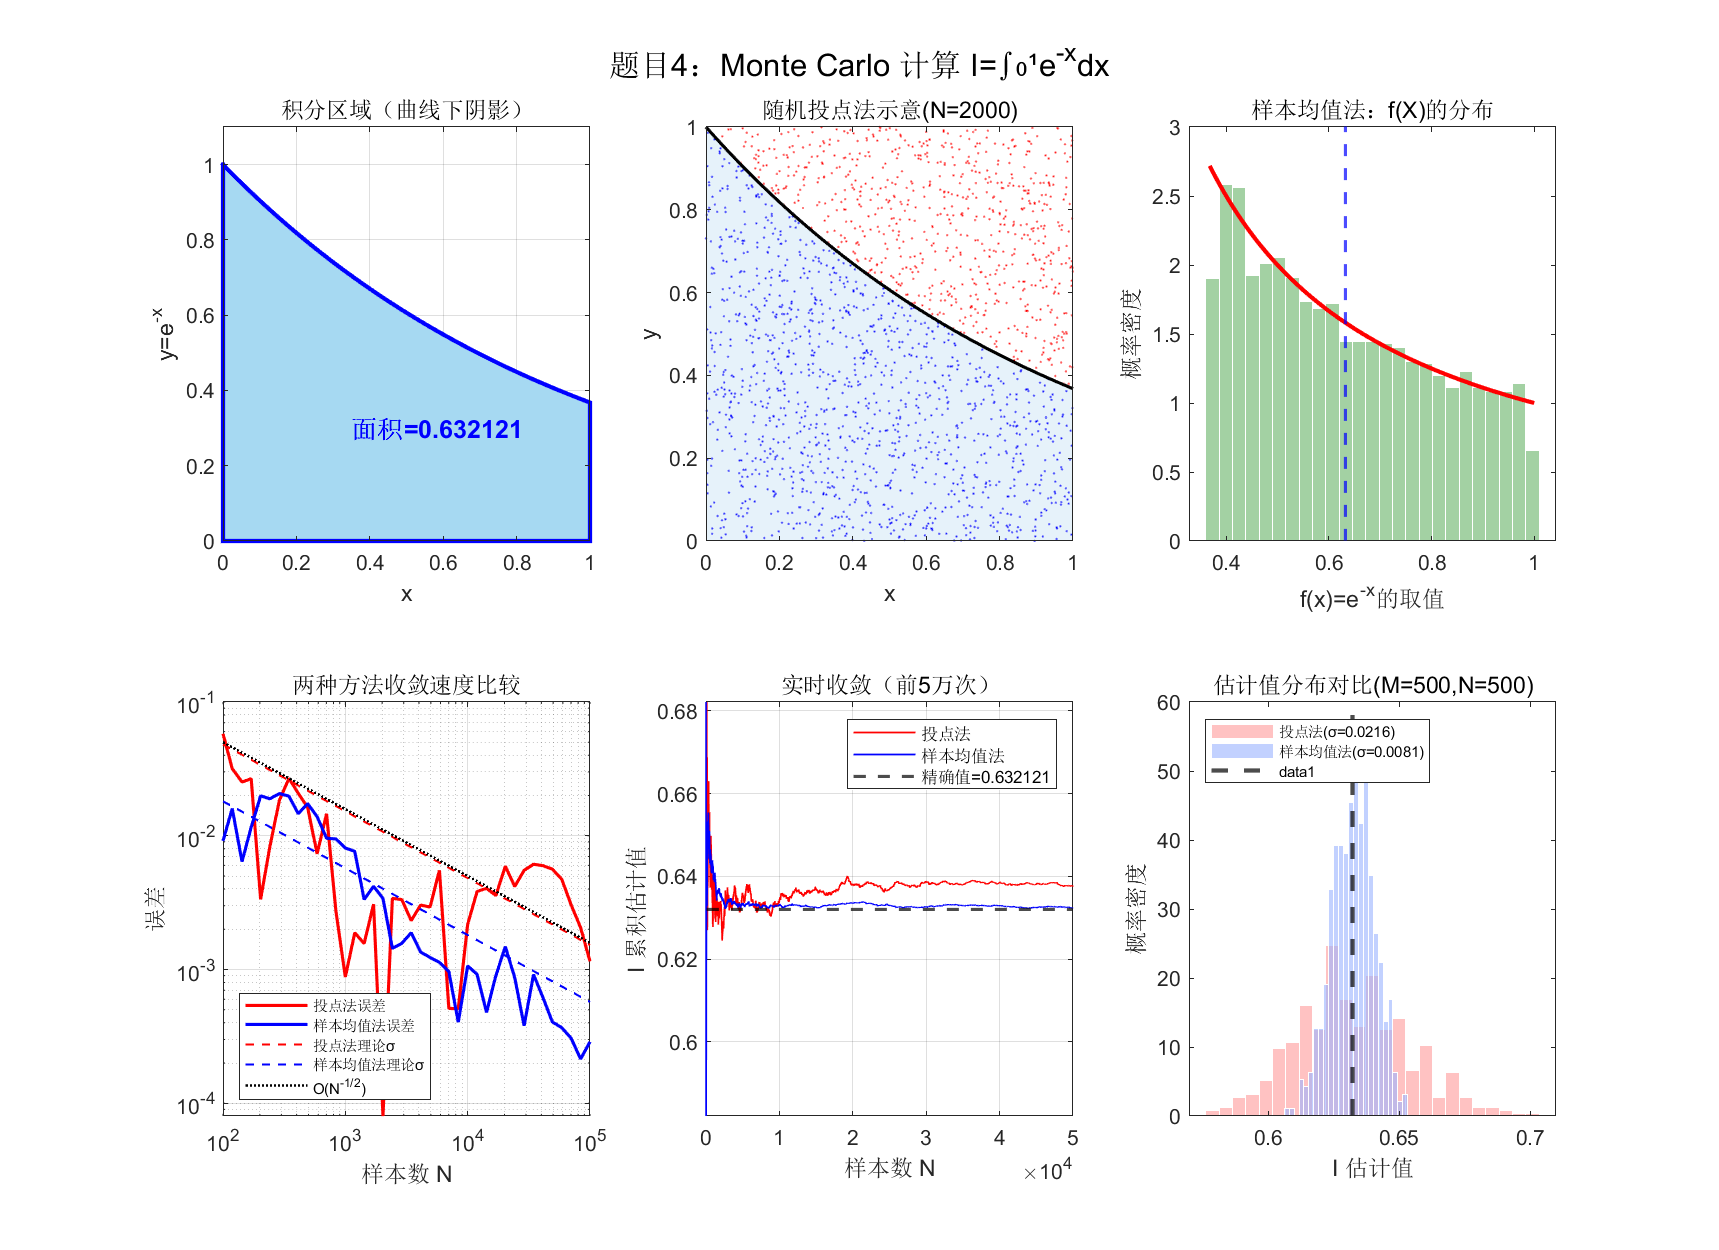
\includegraphics[width=\textwidth]{fig4_monte_carlo.png}
\caption{Monte Carlo 计算 $\int_0^1\mathrm{e}^{-x}\,\mathrm{d}x$ 的结果（$N=5\times10^5$）}
\label{fig:p4}
\end{figure}

\noindent\textbf{大规模计算结果（$N=5\times10^5$）：}

\begin{table}[H]
\centering
\caption{两种 Monte Carlo 方法计算结果比较（$N=5\times10^5$，随机种子 2024）}
\label{tab:p4-results}
\begin{tabular}{lccc}
\toprule
方法 & 估计值 & 绝对误差 & 理论标准差 \\
\midrule
随机投点法（Hit-or-Miss）& $0.633\,224\,000\,0$ & $1.10\times10^{-3}$ & $\approx 6.82\times10^{-4}$ \\
样本均值法（Sample Mean）& $0.632\,206\,478\,5$ & $8.59\times10^{-5}$ & $\approx 2.82\times10^{-4}$ \\
精确值 $1-\mathrm{e}^{-1}$ & $0.632\,120\,558\,829$ & 0 & --- \\
\bottomrule
\end{tabular}
\end{table}

\noindent\textbf{积分区域可视化（图 \ref{fig:p4} 左上图）：}
蓝色阴影区域为 $y=\mathrm{e}^{-x}$ 曲线与 $x$ 轴围成的区域，其面积即为积分值 $I\approx0.6321$．

\noindent\textbf{随机投点法示意（中上图）：}
蓝色点为命中点（落在曲线下方），红色点为未命中点，两者之比近似等于积分值与矩形面积之比．

\noindent\textbf{样本均值法的 $f(X)$ 分布（右上图）：}
$X\sim\mathrm{Uniform}[0,1]$ 时，$f(X)=\mathrm{e}^{-X}$ 的 PDF 为 $1/t$（$t\in[\mathrm{e}^{-1},1]$），
直方图与理论曲线吻合；样本均值即积分估计值，在图中用竖线标注精确值 $I$．

\noindent\textbf{收敛速度比较（左下图）：}
双对数图中两种方法误差均呈 $O(N^{-1/2})$ 的直线，但\textbf{样本均值法的误差曲线始终低于投点法}，
体现了其更小的方差——在相同样本量下精度更高．

\noindent\textbf{实时收敛（中下图）：}
前 $5\times10^4$ 次的累积估计值随 $N$ 的波动幅度，样本均值法（蓝）比投点法（红）波动更小，
更快收敛到精确值（黑色虚线）．

\noindent\textbf{重复实验分布对比（右下图）：}
进行 $M=500$ 次独立实验（每次 $N=500$），投点法（浅红）的分布明显比样本均值法（浅蓝）更宽，
标准差之比约为 $\sqrt{6}\approx2.45$，与理论方差比 $I(1-I)/\mathrm{Var}[f]\approx5.8$ 的平方根吻合．

\subsection{结论}

\begin{itemize}
  \item 两种 Monte Carlo 方法均能无偏估计积分 $I=1-\mathrm{e}^{-1}$，误差均为 $O(N^{-1/2})$；
  \item \textbf{样本均值法}方差约为投点法的 $1/6$，在相同样本量下精度更高、稳定性更好，是 Monte Carlo 积分的首选；
  \item Monte Carlo 方法天然不受维数影响，对高维积分远优于确定性方法（如梯形公式的 $O(N^{-2/d})$ 收敛率），
    但对一维光滑积分，确定性方法（Romberg、自适应 Simpson）效率远高于 Monte Carlo．
\end{itemize}

\clearpage

%% ============================================================
%%  附录
%% ============================================================
\section{附录：程序代码}

\subsection{题目一：数值积分计算 $\pi$（核心部分）}

\begin{lstlisting}[style=matlab, caption={problem1\_pi\_integration.m（核心算法）}]
f = @(x) 4 ./ (1 + x.^2);   % 被积函数 f(x) = 4/(1+x^2)
a = 0; b = 1; pi_exact = pi;

%% 复合梯形公式
% n：子区间数；h：步长；节点 x_i = a + i*h
h_vals = logspace(0, -7, 80);   % 步长序列
for k = 1:length(h_vals)
    n = n_vals(k);
    x_trap = linspace(a, b, n + 1);
    fx_trap = f(x_trap);
    T_n = h_trap/2 * (fx_trap(1) + fx_trap(end) + 2*sum(fx_trap(2:end-1)));
    err_trap(k) = abs(T_n - pi_exact);
end

%% 复合 Simpson 公式
for k = 1:length(h_vals)
    m = max(1, ceil(n/2));
    x_simp = linspace(a, b, 2*m + 1);   % 2m+1 个节点
    fx_simp = f(x_simp);
    % 端点×1；奇数位（中点）×4；偶数内点×2
    S_m = h_simp/3 * (fx_simp(1) + fx_simp(end) + ...
          4*sum(fx_simp(2:2:end-1)) + 2*sum(fx_simp(3:2:end-2)));
    err_simp(k) = abs(S_m - pi_exact);
end

%% Romberg 积分法（Richardson 外推加速）
T = zeros(max_level, max_level);
T(1,1) = (b-a)/2 * (f(a) + f(b));   % 最粗梯形值
for m = 2:max_level
    h_cur = (b-a) / 2^(m-1);
    x_new = a + ((1:2^(m-2)) - 0.5) * (b-a)/2^(m-2);
    T(m,1) = 0.5*T(m-1,1) + h_cur*sum(f(x_new));   % 变步长梯形递推
    for j = 2:m
        c = 4^(j-1);   % Richardson 外推系数
        T(m,j) = (c*T(m,j-1) - T(m-1,j-1)) / (c - 1);
    end
end

%% 自适应 Simpson（递归实现）
function [I, cnt] = adapt_simp(f, a, b, tol, S_ab)
    m = (a+b)/2;
    S_am = simp1(f,a,m);  S_mb = simp1(f,m,b);
    S2 = S_am + S_mb;  cnt = 3;
    err_est = abs(S2 - S_ab) / 15;   % 误差估计（15=4^2-1）
    if err_est <= tol
        I = S2 + (S2 - S_ab)/15;   % Richardson 校正
    else
        [Il,cl] = adapt_simp(f,a,m,tol/2,S_am);   % 递归左半段
        [Ir,cr] = adapt_simp(f,m,b,tol/2,S_mb);   % 递归右半段
        I = Il + Ir;  cnt = cnt + cl + cr;
    end
end
\end{lstlisting}

\subsection{题目二：Planck 积分（核心部分）}

\begin{lstlisting}[style=matlab, caption={problem2\_planck\_integral.m（稳健 Planck 函数）}]
%% 被积函数（数值稳健版本）
function y = planck_func(x)
    if x <= 0
        y = 0;             % f(0) = 0（极限值）
    elseif x > 500
        y = 0;             % 完全衰减
    elseif x > 37          % exp(x) 接近溢出，改用近似
        y = x^3 * exp(-x);   % x^3/(e^x+1) ~= x^3*e^{-x}
    else
        y = x^3 / (exp(x) + 1);   % 正常计算
    end
end

%% 各方法调用（截断区间 [1e-10, 50]）
I_exact = 7 * pi^4 / 120;   % 精确值 7pi^4/120

% 复合梯形（n=5000）
x_trap = linspace(x_min, x_max, n_trap+1);
fx_trap = arrayfun(f_planck, x_trap);
I_trap = h_trap/2*(fx_trap(1)+fx_trap(end)+2*sum(fx_trap(2:end-1)));

% 复合 Simpson（m=2500）
x_simp = linspace(x_min, x_max, 2*m_simp+1);
fx_simp = arrayfun(f_planck, x_simp);
I_simp = h_simp/3*(fx_simp(1)+fx_simp(end)+...
         4*sum(fx_simp(2:2:end-1))+2*sum(fx_simp(3:2:end-2)));
\end{lstlisting}

\subsection{题目三：蒲丰投针（核心部分）}

\begin{lstlisting}[style=matlab, caption={problem3\_buffon\_needle.m（核心算法）}]
rng(42);   % 固定随机种子（可复现）
l = 1.0;  d = 2.0;   % 针长和线间距
N_total = 1e6;

% 生成随机针
y_center = d * rand(1, N_total);     % 中心到最近下方线的距离 ~ Uniform[0,d]
theta    = pi * rand(1, N_total);    % 针与平行线夹角 ~ Uniform[0,pi]

% 判断相交：y < (l/2)*sin(theta) 或 d-y < (l/2)*sin(theta)
half_proj  = (l/2) * sin(theta);
cross_flag = (y_center < half_proj) | (y_center > d - half_proj);
N_cross    = sum(cross_flag);

% 由 P = 2l/(pi*d) 反推 pi
pi_estimate = 2 * l * N_total / (d * N_cross);

% 误差随 N 的收敛分析（利用累积求和避免重复计算）
cumcross = cumsum(cross_flag);
for k = 1:length(N_seq)
    Nk = N_seq(k);
    pi_seq(k) = 2*l*Nk / (d*cumcross(Nk));
    err_seq(k) = abs(pi_seq(k) - pi);
end
\end{lstlisting}

\subsection{题目四：Monte Carlo 积分（核心部分）}

\begin{lstlisting}[style=matlab, caption={problem4\_monte\_carlo.m（核心算法）}]
rng(2024);   % 固定随机种子
f = @(x) exp(-x);   % 被积函数
I_exact = 1 - exp(-1);   % 精确值 1 - 1/e
N_total = 5e5;

%% 随机投点法（Hit-or-Miss）
x_hit = rand(1, N_total);   % x ~ Uniform[0,1]
y_hit = rand(1, N_total);   % y ~ Uniform[0,1]
hits = sum(y_hit <= f(x_hit));   % 判断是否落在曲线下方
I_hitormiss = hits / N_total;    % 矩形面积=1，估计=命中比例
% 理论标准差：sqrt(I*(1-I)/N)

%% 样本均值法（Sample Mean）
x_sample = rand(1, N_total);
I_samplemean = mean(f(x_sample));   % E[f(X)] = I
% 理论标准差：sqrt(Var[f(X)]/N)
% 其中 Var[f] = (1-e^{-2})/2 - I^2 ~= 0.0398（约为投点法的 1/6）

%% 方差比较
fprintf('效率比：投点法方差/样本均值法方差 = %.2f\n', ...
    I_exact*(1-I_exact) / ((1-exp(-2))/2 - I_exact^2));
\end{lstlisting}

\end{document}
